% Options for packages loaded elsewhere
\PassOptionsToPackage{unicode}{hyperref}
\PassOptionsToPackage{hyphens}{url}
%
\documentclass[
]{article}
\usepackage{lmodern}
\usepackage{amsmath}
\usepackage{ifxetex,ifluatex}
\ifnum 0\ifxetex 1\fi\ifluatex 1\fi=0 % if pdftex
  \usepackage[T1]{fontenc}
  \usepackage[utf8]{inputenc}
  \usepackage{textcomp} % provide euro and other symbols
  \usepackage{amssymb}
\else % if luatex or xetex
  \usepackage{unicode-math}
  \defaultfontfeatures{Scale=MatchLowercase}
  \defaultfontfeatures[\rmfamily]{Ligatures=TeX,Scale=1}
  \setmainfont[]{Lato}
\fi
% Use upquote if available, for straight quotes in verbatim environments
\IfFileExists{upquote.sty}{\usepackage{upquote}}{}
\IfFileExists{microtype.sty}{% use microtype if available
  \usepackage[]{microtype}
  \UseMicrotypeSet[protrusion]{basicmath} % disable protrusion for tt fonts
}{}
\makeatletter
\@ifundefined{KOMAClassName}{% if non-KOMA class
  \IfFileExists{parskip.sty}{%
    \usepackage{parskip}
  }{% else
    \setlength{\parindent}{0pt}
    \setlength{\parskip}{6pt plus 2pt minus 1pt}}
}{% if KOMA class
  \KOMAoptions{parskip=half}}
\makeatother
\usepackage{xcolor}
\IfFileExists{xurl.sty}{\usepackage{xurl}}{} % add URL line breaks if available
\IfFileExists{bookmark.sty}{\usepackage{bookmark}}{\usepackage{hyperref}}
\hypersetup{
  hidelinks,
  pdfcreator={LaTeX via pandoc}}
\urlstyle{same} % disable monospaced font for URLs
\usepackage[margin=1in]{geometry}
\usepackage{graphicx}
\makeatletter
\def\maxwidth{\ifdim\Gin@nat@width>\linewidth\linewidth\else\Gin@nat@width\fi}
\def\maxheight{\ifdim\Gin@nat@height>\textheight\textheight\else\Gin@nat@height\fi}
\makeatother
% Scale images if necessary, so that they will not overflow the page
% margins by default, and it is still possible to overwrite the defaults
% using explicit options in \includegraphics[width, height, ...]{}
\setkeys{Gin}{width=\maxwidth,height=\maxheight,keepaspectratio}
% Set default figure placement to htbp
\makeatletter
\def\fps@figure{htbp}
\makeatother
\setlength{\emergencystretch}{3em} % prevent overfull lines
\providecommand{\tightlist}{%
  \setlength{\itemsep}{0pt}\setlength{\parskip}{0pt}}
\setcounter{secnumdepth}{-\maxdimen} % remove section numbering
\usepackage{array}
\usepackage{enumitem}
\usepackage{longtable}
\usepackage{graphicx}
\usepackage{fontspec}
\usepackage{fontawesome}
\usepackage{tabularx}
\usepackage{fullpage,graphicx,tikz}
\usepackage{tikzpagenodes}
\usepackage{fancyhdr}
\usepackage{xcolor}
\usepackage{hyperref}
\ifluatex
  \usepackage{selnolig}  % disable illegal ligatures
\fi

\author{}
\date{\vspace{-2.5em}}

\begin{document}

\definecolor{downloadcolor}{RGB}{30, 135, 240}
\definecolor{mygray}{RGB}{153, 153, 153}
\usetikzlibrary{calc}

\pagestyle{fancy}
\fancyhf{}
\lfoot{\textcolor{mygray}{\textit{December, 2020}}}
\cfoot{\textcolor{mygray}{\textit{Ethan S. Young $\cdot$ Curriculum Vitae}}}
\rfoot{\textcolor{mygray}{\textit{\thepage}}}
\renewcommand{\headrulewidth}{0pt}

\begin{center}
  \Huge{\textbf{\textit{Ethan S. Young}}} \\
\end{center}

\vspace{2ex}

\begin{minipage}{5cm}
  \begin{center}
    Postdoctoral Researcher \\
    Department of Pyschology, Utrecht University \\
    Utrecht, The Netherlands \\
  \end{center}
\end{minipage}
\hfill
\begin{minipage}{5cm}
  \begin{tikzpicture}[baseline=(ola.center),inner sep=0pt]
    \clip (0,0)  circle (2.25cm) node (ola) {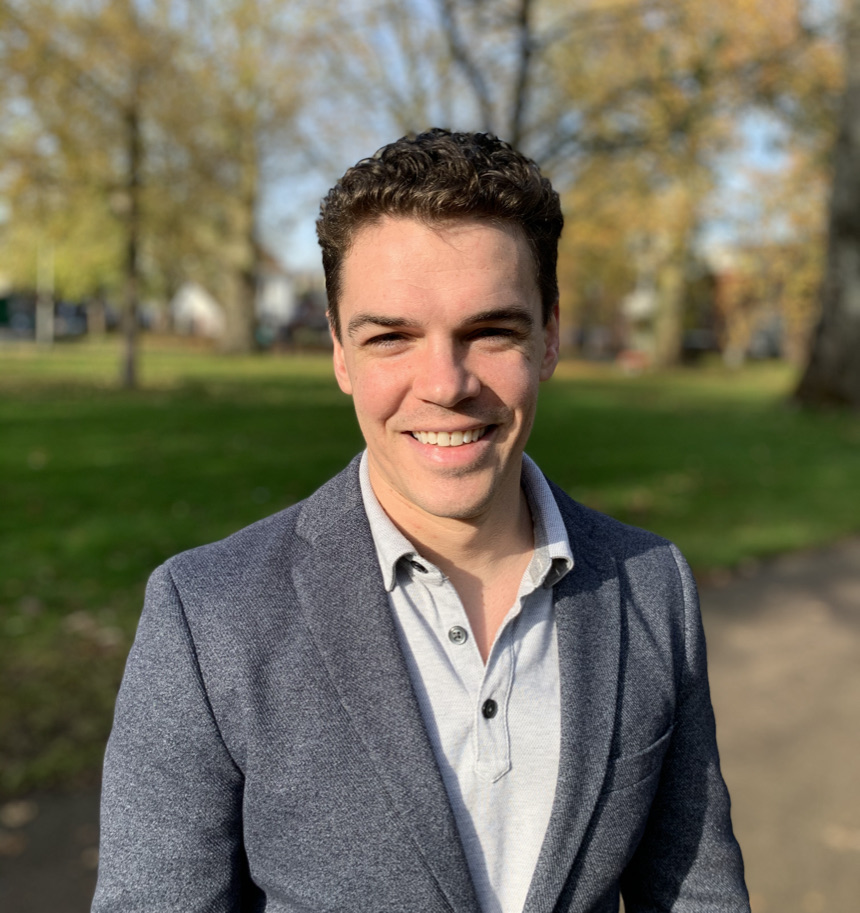
\includegraphics[width=4.5cm]{pic1.jpeg}};
  \end{tikzpicture}
\end{minipage}
\hfill
\begin{minipage}{5cm}
  \faPhone{} +31 6 82583068  \\
  \faEnvelope{} \href{mailto:young.ethan.scott@gmail.com}{young.ethan.scott@gmail.com}\\
  \faHome{} \href{www.ethan-young.com}{ethan-young.com} \\
  \faGithub{} \href{https://github.com/ethan-young}{github}\\
\end{minipage}

\vspace{1ex}

\hypertarget{education}{%
\section{\texorpdfstring{\textbf{Education}}{Education}}\label{education}}

\vspace{1ex}
\begin{color}{mygray}\hrule\end{color}
\vspace{1ex}

\begin{longtable}{p{2.25cm}p{5.5in}}
2019 & \parbox[t]{5.0in}{Doctorate of Philosophy \newline University of Minnesota \newline Psychology} \\\\& \\
2017 & \parbox[t]{5.0in}{Master's of Arts \newline University of Minnesota \newline Psychology} \\\\& \\
2012 & \parbox[t]{5.0in}{Bachelor's of Arts \newline University of Minnesota \newline Psychology} \\
\end{longtable}

\vspace{1ex}

\hypertarget{academic-positions}{%
\section{\texorpdfstring{\textbf{Academic
Positions}}{Academic Positions}}\label{academic-positions}}

\vspace{1ex}
\begin{color}{mygray}\hrule\end{color}
\vspace{1ex}

\begin{longtable}{p{2.25cm}p{5.5in}}
2020-2022 & \parbox[t]{5.0in}{Postdoctoral Researcher \newline Utrecht University \newline advisors: Dr. Willem Frankenhuis} \\\\& \\
2019-2020 & \parbox[t]{5.0in}{Postdoctoral Researcher \newline Radboud University \newline advisors: Dr. Willem Frankenhuis} \\\\& \\
2013-2019 & \parbox[t]{5.0in}{PhD Student \newline University of Minnesota \newline advisors: Drs. Jeffry Simpson \& Vladas Griskevicius} \\\\& \\
2012-2016 & \parbox[t]{5.0in}{Graduate Research Assistant \newline University of Minnesota \newline advisors: Drs. Jeffry Simpson \& Glenn Roisman} \\\\& \\
2012-2013 & \parbox[t]{5.0in}{Graduate Research Assistant \newline University of Minnesota \newline advisors: Drs. Jeffry Simpson \& Vladas Griskevicius} \\\\& \\
2012-2013 & \parbox[t]{5.0in}{Lab Manager \newline University of Minnesota \newline advisors: Dr. Kathleen Vohs} \\
\end{longtable}

\vspace{1ex}

\hypertarget{honors-awards}{%
\section{\texorpdfstring{\textbf{Honors \&
Awards}}{Honors \& Awards}}\label{honors-awards}}

\vspace{1ex}
\begin{color}{mygray}\hrule\end{color}
\vspace{1ex}

\hypertarget{awards}{%
\subsection{\texorpdfstring{\emph{Awards}}{Awards}}\label{awards}}

\begin{longtable}{p{2.25cm}p{5.5in}}
2019 & \parbox[t]{5.0in}{Best Article of the Year Award \newline Childhood attachment and adult personality: a life history perspective. \newline \textit{Self \& Identity}} \\
\end{longtable}

\hypertarget{fellowships}{%
\subsection{\texorpdfstring{\emph{Fellowships}}{Fellowships}}\label{fellowships}}

\begin{longtable}{p{2.25cm}p{5.5in}}
2018-2019 & \parbox[t]{5.0in}{Doctoral Dissertation Fellowship \newline University of Minnesota} \\\\& \\
2017-2018 & \parbox[t]{5.0in}{Thomas J. Bouchard Fellowship \newline University of Minnesota} \\
\end{longtable}

\vspace{1ex}

\hypertarget{publications}{%
\section{\texorpdfstring{\textbf{Publications}}{Publications}}\label{publications}}

\vspace{1ex}
\begin{color}{mygray}\hrule\end{color}
\vspace{1ex}

\hypertarget{peer-reviewed-papers}{%
\subsection{\texorpdfstring{\emph{Peer-Reviewed
Papers}}{Peer-Reviewed Papers}}\label{peer-reviewed-papers}}

\noindent 

\begin{longtable}{p{2.25cm}p{5.5in}}
2020 & \hangindent=0.25cm \textbf{Young, E. S.}, Frankenhuis, W. E., \& Ellis, B. J. (2020). Theory and measurement of environmental harshness and unpredictability. \textit{Evolution and Human Behavior}. \newline \href{https://www.ethan-young.com/publications/journal/2020_EHB_Young.pdf}{\textcolor{downloadcolor}{\faFilePdfO{} View}} \\ \\& \\[-1.5em]
 & \hangindent=0.25cm \textbf{Young, E. S.}, Doom, J. R., Farrell, A. K., Carlson, E. A., Englund, M. M., Miller, G. E., Gunnar, M. R., Roisman, G. I., \& Simpson, J. A. (2020). Life stress and cortisol reactivity: An exploratory analysis of stress exposure across life on HPA axis functioning. \textit{Development and Psychopathology}. \newline \href{https://www.ethan-young.com/publications/journal/2020_DP_Young.pdf}{\textcolor{downloadcolor}{\faFilePdfO{} View}} \\ \\& \\[-1.5em]
 & \hangindent=0.25cm Waters, T. E., Facompré, C. R., Dagan, O., Martin, J., Johnson, W. F., \textbf{Young, E. S.}, Jessica Shankman, Yoojin Lee, Jeffry A. Simpson, and Glenn I. Roisman. (2020). Convergent validity and stability of secure base script knowledge from young adulthood to midlife. Attachment \& Human Development. \newline \href{https://www.ethan-young.com/publications/journal/2020_AHD_Waters.pdf}{\textcolor{downloadcolor}{\faFilePdfO{} View}} \\ \\& \\[-1.5em]
 & \hangindent=0.25cm Frankenhuis, W. E., \textbf{Young, E. S.}, \& Ellis, B. J. (2020). The hidden talents approach: Theoretical and methodological challenges. \textit{Trends in Cognitive Sciences}, 24, 569-581. \newline \href{https://www.ethan-young.com/publications/journal/2020_TICS_Frankenhuis.pdf}{\textcolor{downloadcolor}{\faFilePdfO{} View}} \\ \\& \\[-1.5em]
2019 & \hangindent=0.25cm \textbf{Young, E. S.}, Farrell, A. K., Carlson, E. A., Englund, M. M., Miller, G. E., Gunnar, M. R., Roisman, G. I., \& Simpson, J. A. (2019). The dual impact of early and concurrent life stress on adults’ diurnal cortisol patterns: A prospective study. \textit{Psychological Science}, 30, 739-747. \newline \href{https://www.ethan-young.com/publications/journal/2019_PS_Young.pdf}{\textcolor{downloadcolor}{\faFilePdfO{} View}} \\ \\& \\[-1.5em]
 & \hangindent=0.25cm \textbf{Young, E. S.}, Simpson, J. A., Griskevicius, V., Huelsnitz, C. O., \& Fleck, C. (2019). Childhood attachment and adult personality: a life history perspective. \textit{Self and Identity}, 18(1), 22-38. \newline \href{https://www.ethan-young.com/publications/journal/2019_SI_Young.pdf}{\textcolor{downloadcolor}{\faFilePdfO{} View}} \\ \\& \\[-1.5em]
 & \hangindent=0.25cm Farrell, A. K., Waters, T. E., \textbf{Young, E. S.}, Englund, M. M., Carlson, E. A., Roisman, G. I., \& Simpson, J. (2019). Early maternal sensitivity, attachment security in young adulthood, and cardiometabolic risk at midlife. \textit{Attachment and Human Development}, 21(1), 70-86. \newline \href{https://www.ethan-young.com/publications/journal/2019_AHD_Farrell.pdf}{\textcolor{downloadcolor}{\faFilePdfO{} View}} \\ \\& \\[-1.5em]
2018 & \hangindent=0.25cm \textbf{Young, E. S.}, Griskevicius, V., Simpson, J. A., Waters, T. E. A., \& Mittal, C. (2018). Can an Unpredictable Childhood Environment Enhance Working Memory? Testing the Sensitized-Specialization Hypothesis. \textit{Journal of Personality and Social Psychology}, 114(6), 891–908. \newline \href{https://www.ethan-young.com/publications/journal/2018_JPSP_Young.pdf}{\textcolor{downloadcolor}{\faFilePdfO{} View}} \\ \\& \\[-1.5em]
 & \hangindent=0.25cm Martin, J., Anderson, J. E., Groh, A. M., Waters, T. E. A., \textbf{Young, E. S.}, Johnson, W. F., … Roisman, G. I. (2018). Maternal Sensitivity During the First 3 1/2 Years of Life Predicts Electrophysiological Responding to and Cognitive Appraisals of Infant Crying at Midlife. \textit{Developmental Psychology}, 54(10), 1917–1927. \newline \href{https://www.ethan-young.com/publications/journal/2018_DP_Martin.pdf}{\textcolor{downloadcolor}{\faFilePdfO{} View}} \\ \\& \\[-1.5em]
2017 & \hangindent=0.25cm Szepsenwol, O., Griskevicius, V., Simpson, J. A., \textbf{Young, E. S.}, Fleck, C., \& Jones, R. E. (2017). The effect of predictable early childhood environments on sociosexuality in early adulthood. \textit{Evolutionary Behavioral Sciences}, 11(2), 131 \newline \href{https://www.ethan-young.com/publications/journal/2017_EBS_Szepsenwol.pdf}{\textcolor{downloadcolor}{\faFilePdfO{} View}} \\ \\& \\[-1.5em]
2015 & \hangindent=0.25cm Mittal, C., Griskevicius, V., Simpson, J. A., Sung, S., \& \textbf{Young, E. S.} (2015). Cognitive Adaptations to Stressful Environments: When Childhood Adversity Enhances Adult Executive Function. \textit{Journal of Personality and Social Psychology}, 109(4), 604–621. \newline \href{https://www.ethan-young.com/publications/journal/2015_JPSP_Mittal.pdf}{\textcolor{downloadcolor}{\faFilePdfO{} View}} \\ 
\end{longtable}

\hypertarget{book-chapters}{%
\subsection{\texorpdfstring{\emph{Book
Chapters}}{Book Chapters}}\label{book-chapters}}

\noindent 

\begin{longtable}{p{2.25cm}p{5.5in}}
2020 & \hangindent=0.25cm \textbf{Young, E. S.}, \& Simpson, J. A. (2020). An evolutionary, life history perspective on relationship maintenance. In B. G. Ogolsky \& J. K. Monk (Eds.), Relationship maintenance: Theory, process, and context (pp. 29-46). New York, NY: Cambridge University Press. \newline \href{https://www.ethan-young.com/cv/chapter/2019_Young_maintenance.pdf}{\textcolor{downloadcolor}{\faFilePdfO{} View}} \\ \\& \\[-1.5em]
2017 & \hangindent=0.25cm Simpson, J. A., Griskevicius, V., Szepsenwol, O., \& \textbf{Young, E. S.} (2017). An evolutionary life history perspective on personality and mating strategies. In A. T. Church (Ed.), The Praeger handbook of personality across cultures. Volume 3: Evolutionary, ecological, and cultural contexts of personality (pp. 1-29). Santa Barbara, CA: Praeger. \newline \href{https://www.ethan-young.com/cv/chapter/2017_chapter_Simpson_LHTpersonality.pdf}{\textcolor{downloadcolor}{\faFilePdfO{} View}} \\ 
\end{longtable}

\hypertarget{in-progress}{%
\subsection{\texorpdfstring{\emph{In
Progress}}{In Progress}}\label{in-progress}}

\noindent 

\begin{longtable}{p{2.25cm}p{5.5in}}
in progress & \hangindent=0.25cm \textbf{Young, E. S.}, Frankenhuis, W. E., \& Ellis, B. J. Adversity, Memory Updating, and Attention Shifting: Do real-world stimuli help or hurt performance? \\ 
\end{longtable}

\vspace{1ex}

\hypertarget{presentations}{%
\section{\texorpdfstring{\textbf{Presentations}}{Presentations}}\label{presentations}}

\vspace{1ex}
\begin{color}{mygray}\hrule\end{color}
\vspace{1ex}

\hypertarget{talks-first-author-only}{%
\subsection{\texorpdfstring{\emph{Talks (first author
only)}}{Talks (first author only)}}\label{talks-first-author-only}}

\noindent 

\begin{longtable}{p{2.25cm}p{5.5in}}
2019 & \hangindent=0.25cm \textbf{Young, E. S.}, Griskevicius, V., Simpson, J. A., Waters, T. E. A., \& Mittal, C. (2019, February). Can an Unpredictable Childhood Environment Enhance Working Memory? Testing the Sensitized-Specialization Hypothesis. Presented at Society for Personality and Social Psychology, Portland, OR. \newline \href{https://www.ethan-young.com/cv/conference/2019_SPSP_talk.pdf}{\textcolor{downloadcolor}{\faFilePdfO{} View}} \\ \\& \\[-1.5em]
2018 & \hangindent=0.25cm \textbf{Young, E. S.}, Griskevicius, V., Simpson, J. A., Waters, T. E. A., \& Mittal, C. (2018, October). Can an Unpredictable Childhood Environment Enhance Working Memory? Testing the Sensitized-Specialization Hypothesis. Presented at Society for Research in Child Development - Special Topics Meeting on Character Development, Philadelphia, PA. \newline \href{https://www.ethan-young.com/cv/conference/2018_SRCD_CD_talk.pdf}{\textcolor{downloadcolor}{\faFilePdfO{} View}} \\ \\& \\[-1.5em]
2017 & \hangindent=0.25cm \textbf{Young, E. S.}, Griskevicius, V., Simpson, J. A., Waters, T. E. A., \& Mittal, C. (2017, May). Can an Unpredictable Childhood Environment Enhance Working Memory? Testing the Sensitized-Specialization Hypothesis. Presented at Human Behavior and Evolution Society, Boise, ID. \newline \href{https://www.ethan-young.com/cv/conference/2017_HBES_talk.pdf}{\textcolor{downloadcolor}{\faFilePdfO{} View}} \\ 
\end{longtable}

\hypertarget{posters-first-author-only}{%
\subsection{\texorpdfstring{\emph{Posters (first author
only)}}{Posters (first author only)}}\label{posters-first-author-only}}

\noindent 

\begin{longtable}{p{2.25cm}p{5.5in}}
 2019 &\hangindent=0.25cm \textbf{Young, E. S.}, Griskevicius, V., Simpson, J. A., Waters, T. E. A., \& Mittal, C. (2019, November). Can an unpredictable childhood environment enhance aspects of executive function and working memory? Poster Presented at The Cognition, Behavior \& Evolution Network, Amsterdam, NL. \newline \href{https://www.ethan-young.com/cv/conference/2019_CBEN_poster.pdf}{\textcolor{downloadcolor}{\faFilePdfO{} View}} \\ \\& \\[-1.5em]
 2015 &\hangindent=0.25cm \textbf{Young, E. S.}, Griskevicius, V., Simpson, J. A., Waters, T. E. A., \& Mittal, C. (2015, February). Cognitive Specialization of Memory: Early life stress enhances working memory in the face of economic uncertainty. Poster presented at Society for Personality and Social Psychology, Long Beach, CA. \newline \href{https://www.ethan-young.com/cv/conference/2015_SPSP_poster.pdf}{\textcolor{downloadcolor}{\faFilePdfO{} View}} \\ \\& \\[-1.5em]
  &\hangindent=0.25cm \textbf{Young, E. S.}, Griskevicius, V., Simpson, J. A., Waters, T. E. A., \& Mittal, C. (2015, May). Cognitive Specialization of Memory: Early life stress enhances working memory in the face of economic uncertainty. Poster presented at Human Behavior and Evolution Society, Columbia, MO. \newline \href{https://www.ethan-young.com/cv/conference/2015_HBES_poster.pdf}{\textcolor{downloadcolor}{\faFilePdfO{} View}} \\ \\& \\[-1.5em]
 2013 &\hangindent=0.25cm \textbf{Young, E. S.}, Mittal, C., Griskevicius, V., \& Simpson, J. A. (2013, July). Biological Sensitivity to Context and Life History Theory: How the same trait leads to different behavior. Poster presented at Human Behavior and Evolution Society, South Beach Miami, FL. \newline \href{https://www.ethan-young.com/cv/conference/2013_HBES_poster.pdf}{\textcolor{downloadcolor}{\faFilePdfO{} View}} \\ 
\end{longtable}

\vspace{1ex}

\hypertarget{teaching-mentoring}{%
\section{\texorpdfstring{\textbf{Teaching \&
Mentoring}}{Teaching \& Mentoring}}\label{teaching-mentoring}}

\vspace{1ex}
\begin{color}{mygray}\hrule\end{color}
\vspace{1ex}

\hypertarget{instructor}{%
\subsection{\texorpdfstring{\emph{Instructor}}{Instructor}}\label{instructor}}

\begin{longtable}{p{2.25cm}p{5.5in}}
 Fall 2017 & Introduction to Individual Differences (Psy 3135) \newline University of Minnesota \\
\end{longtable}

\hypertarget{section-leader}{%
\subsection{\texorpdfstring{\emph{Section
Leader}}{Section Leader}}\label{section-leader}}

\begin{longtable}{p{2.25cm}p{5.5in}}
 Spring 2018 & Introduction to Psychological Measurement and Data Analysis (Psy 3801) \newline University of Minnesota \\\\& \\
 Spring 2017 & Introduction to Psychological Measurement and Data Analysis (Psy 3801) \newline University of Minnesota \\\\& \\
 Fall 2016 & Introduction to Psychological Measurement and Data Analysis (Psy 3801) \newline University of Minnesota \\
\end{longtable}

\hypertarget{teaching-assistant}{%
\subsection{\texorpdfstring{\emph{Teaching
Assistant}}{Teaching Assistant}}\label{teaching-assistant}}

\begin{longtable}{p{2.25cm}p{5.5in}}
 Spring 2018 & Honors Practicum (Psy 4993V) \newline University of Minnesota \\\\& \\
 Spring 2017 & Introduction to Individual Differences (Psy 3135) \newline University of Minnesota \\\\& \\
 Fall 2016 & Introduction to Individual Differences (Psy 3135) \newline University of Minnesota \\
\end{longtable}

\vspace{1ex}

\hypertarget{ad-hoc-reviewing}{%
\section{\texorpdfstring{\textbf{Ad Hoc
Reviewing}}{Ad Hoc Reviewing}}\label{ad-hoc-reviewing}}

\vspace{1ex}
\begin{color}{mygray}\hrule\end{color}
\vspace{1ex}

\begin{itemize}
\tightlist
\item
  \emph{Child Development}
\item
  \emph{Evolution and Human Behavior}
\item
  \emph{Evolutionary Psychology}
\item
  \emph{Personality and Social Psychology Bulletin}
\item
  \emph{Journal of Child Psychology and Psychiatry}
\end{itemize}

\vspace{1ex}

\hypertarget{professional-memberships}{%
\section{\texorpdfstring{\textbf{Professional
Memberships}}{Professional Memberships}}\label{professional-memberships}}

\vspace{1ex}
\begin{color}{mygray}\hrule\end{color}
\vspace{1ex}

\begin{itemize}
\tightlist
\item
  Society for Personality and Social Psychology (SPSP)
\item
  Human Behavior and Evolution Society (HBES)
\end{itemize}

\end{document}
